\documentclass{amsart}
\usepackage{fullpage}

\usepackage[T1]{fontenc}
\usepackage[utf8]{inputenc} 
\usepackage{lmodern}
\usepackage[slovene]{babel}
\usepackage{hyperref}
\usepackage{amsmath,amssymb,amsfonts, mathtools}
\usepackage{bbm}
\usepackage{graphicx}
\graphicspath{{./images/}}

\linespread{1.2}

\newcommand{\N}{\mathbb{N}}
\newcommand{\Z}{\mathbb{Z}}
\newcommand{\Q}{\mathbb{Q}}
\newcommand{\R}{\mathbb{R}}
\newcommand{\C}{\mathbb{C}}

% tekst napisan pokoncno
\theoremstyle{definition}
\newtheorem{definicija}{Definicija}[section]
\newtheorem{primer}[definicija]{Primer}
\newtheorem{opomba}[definicija]{Opomba}

\renewcommand\endprimer{\hfill$\diamondsuit$}

\theoremstyle{plain} % tekst napisan posevno
\newtheorem{lema}[definicija]{Lema}
\newtheorem{izrek}[definicija]{Izrek}
\newtheorem{trditev}[definicija]{Trditev}
\newtheorem{posledica}[definicija]{Posledica}

\newcommand\Vtextvisiblespace[1][.3em]{%
\mbox{\kern.06em\vrule height.3ex}%
\vbox{\hrule width#1}%
\hbox{\vrule height.3ex}}

\title{Kontekstno-neodvisne gramatike za kodiranje in stiskanje podatkov}
\author{Janez Podlogar}
\date{\today}

\begin{document}

\begin{abstract}

    V delu podamo definicje kodiranja, dekodiranja in stiskanja podtakov ter predstavimo
    primere, ki motivirajo stiskanje podatkov s kontekstno-neodvisnimi gramatikami.

\end{abstract}

\maketitle

\section{Kodiranje podatkov}

Zapis informacije v neki obliki ni primeren za vsakršno rabo. Besedilo, zapisano z 
pismenkami, je neberljivo za slepe osebe, saj je komunikacijski kanal v tem primeru
vid. Prav tako pisanega besedila v prvotni obliki ni mogoče poslati s telegrafom. V tem
primeru je komunikacijski kanal žica in pismenke se po njej ne morejo sprehoditi. V obeh 
primerih je informacija, ki bi jo radi prenesli, zapisana v neprimerni obliki. V prvem 
primeru je potrebno besedilo zapisati z Braillovo pisavo. V drugem primeru pa je
besedilo potrebno pretvoriti v električni signal. Spreminjanje zapisa sporočila
imenujemo \textit{kodiranje}, sistemu pravil, po katerem se kodiranje opravi,
pa \textit{kod}.

\begin{primer}\label{Morse}

    \textit{Morsejeva abeceda} je kodiranje črk, števil in ločil s pomočjo zaporedja kratkih
    in dolgih signalov:

    \begin{itemize}
        \item Dolžina kratkega signala je ena enota.
        \item Dolgi signal je trikrat daljši od kratkega signala.
        \item Razmik med signali znotraj črke je tišina dolžine kratkega signala.
        \item Razmik med črkami je tišina dolga tri kratke signale oziroma en dolgi signal.
        \item Presledek med besedami je tišina dolga sedem kratkih signalov.
    \end{itemize}

    \begin{figure}[h]
        \centering
        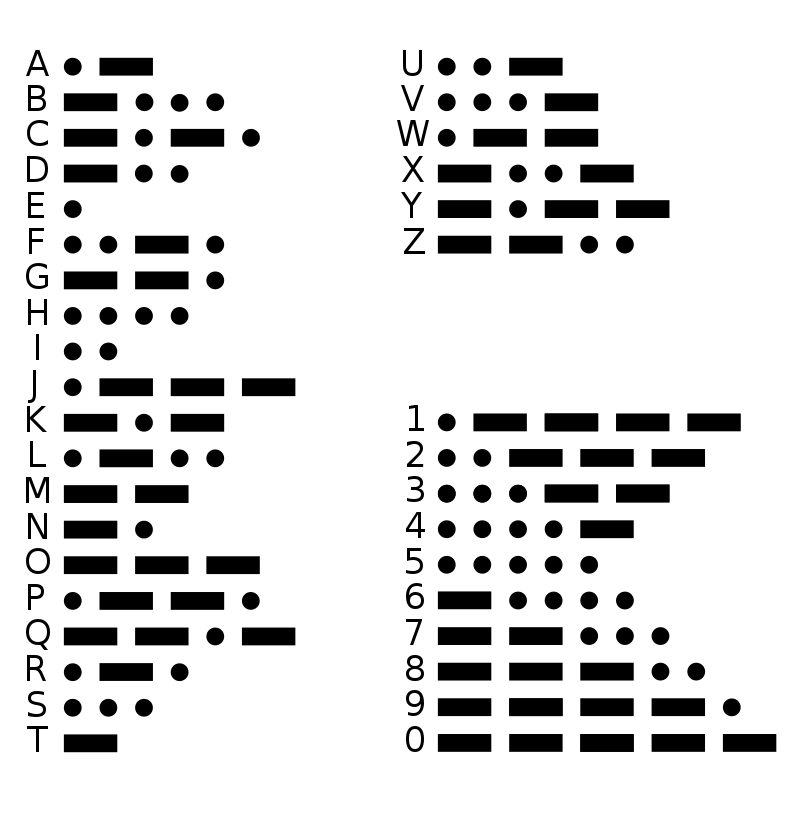
\includegraphics[width=4.3cm]{International_Morse_Code.svg.png}
        \caption{Mednarodna Morsejeva abeceda.}
        \label{fig:Morse}
    \end{figure}

    Prvotni namen Morsejeve abecede je komunikacija preko telegrama, saj komunikacijski
    kanal dovoljuje le električne signale in tišino med njimi. Kodiranje črk je takšno,
    da imajo črke z višjo frekvenco (v angleškem jeziku) krajši zapis. Tako se koda
    sporočila skrajša in posledično tudi čas njegovega prenosa.

\end{primer}

\begin{definicija}

    \textit{Abeceda} je končna neprazna množica $ \Sigma $. Elementom abecede pravimo \textit{črke}.
    \textit{Množica vseh končnih nizov abecede} $ \Sigma $ je
    \[
        \Sigma^* = \{ a_1 a_2 a_3 \cdots a_n \mid n \in \N_0 \land \forall i: a_i \in \Sigma \}, 
    \]
    kjer za $ n = 0 $ dobimo prazen niz, ki ga označimo z $ \varepsilon $.
    \textit{Dolžino niza w} označimo z $ |w| $ in je enaka številu črk v nizu $ w \in \Sigma^* $.
    \textit{Jezik na abecedi} $ \Sigma $ je poljubna podmnožica množice $ \Sigma^* $. 

\end{definicija}

\begin{opomba}
    
    \textit{Kleenejeva zvezdica} ali \textit{Kleenejevo zaprtje} je operacija, ki
    abecedi $ \Sigma $ priredi najmanjšo nadmnožico $ \Sigma^* $, ki vsebuje
    \textit{prazen niz} $ \varepsilon $ in je zaprta za operacijo stikanje, ki ji
    pravimo tudi konkatenacijo oziroma veriženje. Element $ \varepsilon $ je
    nevtralni element za stikanje. Z drugimi besedami, $ \Sigma^* $ je množica vseh
    končnih nizov, ki jih lahko generiramo z veriženjem črk abecede $ \Sigma $. \\
    Za abecedo $ \Sigma $ definirajmo
    \[
        \Sigma^0 = \{ \varepsilon \}
    \]
    ter za vsak $ \ell > 0 $ rekurzivno
    \[
        \Sigma^{\ell+1} = \{ wa \mid w \in \Sigma^{\ell} \text{ in } a \in \Sigma \}.
    \]
    Potem je Kleenejeva zvezdico na $ \Sigma $ enaka
    \[
        \Sigma^* = \bigcup_{\ell \geq 0} \Sigma^\ell.
    \]
    Omenimo še, da je $ \Sigma^{\ell} $ množica vseh nizov abecede $ \Sigma $ dolžine $ \ell $.

\end{opomba}

\begin{primer}
    
    Naj bo $ \Sigma = \{ a,b,c \} $ abeceda, potem so $ \mathit{ab}, \mathit{ccc} \text{ in }
    \mathit{cababcccababcccab} $ končni nizi abecede $ \Sigma $ in potemtakem elementi $ \Sigma^* $.

\end{primer}

\begin{definicija}
    
    \textit{Kodiranje nizov abecede} $ \Sigma $ je injektivna funkcija $ \kappa \colon \Sigma^* 
    \to \Sigma_c^* $, kjer imenujemo $ \Sigma_c $ \textit{kodna abeceda} in $ \kappa(w) $ 
    \textit{koda niza} $ w $. \textit{Dokodiranje kodiranja} $ \kappa $ je funkcija 
    $ \delta \colon C \subseteq \Sigma^*_c \to \Sigma^* $, da velja
    \[
        \forall w \in \Sigma^* \colon \delta(\kappa(w)) = w.
    \]

\end{definicija}

\begin{opomba}
    
    Funkcijo $ \kappa $ imenujemo \textit{kodna funkcija}, funkcijo $ \delta $ pa
    \textit{dekodna funckija}.

\end{opomba}

\begin{opomba}
    
    Zožitev kodomene kodne funkcije $ \kappa $ na $ C \subseteq \Sigma^*_c $ je bijektivna funkcija.

\end{opomba}

\begin{primer}
    
    Formalizirajmo Morsejevo abecedo iz Primera~\refeq{Morse}. Abecedi sta
    \[
        \Sigma = \{ \text{A},  \text{B}, \ldots, \text{Z} \} \cup \{ 0, 1, \ldots, 9 \}
        \cup \{ \Vtextvisiblespace[5pt] \}, \quad
        \Sigma_c = \{ \cdot ,-, \Box \},
    \]
    kjer je \Vtextvisiblespace[5pt] presledek in $ \Box $ ena kratka enota tišine. Definirajmo kodno
    funkcijo črk abecede $ \kappa_s \colon \Sigma \to \Sigma_c^* $, ki vsaki črki iz abecede $ \Sigma_s $
    priredi niz črk kodne abecede $ \Sigma_c $. Predpis funkcije $ \kappa_s $ je določen s tabelo iz 
    Slike~\refeq{fig:Morse}, dodatno presledek \Vtextvisiblespace[5pt] kodiramo v tri kratkih enot tišine
    \[
        \kappa_s(\Vtextvisiblespace[5pt]) = \Box\Box\Box\Box.
    \]
    Za niz $ w = a_1a_2 \ldots a_n \in \Sigma^* $ definiramo kodno 
    funkcijo $ K $ po črkah
    \[
        \kappa(w) = \kappa_s(a_1) \Box\Box\Box \kappa_s(a_2) \Box\Box\Box \cdots \kappa_s(a_n).
    \]
    Poglejmo si dva primera kodiranja v Morsejevi abecedi
    \begin{gather*}
        \kappa(\text{SOS}) = \phantom{} \cdot\Box\cdot\Box\cdot \Box\Box\Box -\Box-\Box- \Box\Box\Box \cdot\Box\cdot\Box\cdot \phantom{}, \\
        \kappa(\text{AD\Vtextvisiblespace[5pt]HOC}) = \phantom{} \cdot\Box- \Box\Box\Box -\Box\cdot\Box\cdot 
        \Box\Box\Box\Box\Box\Box\Box
        \cdot\Box\cdot\Box\cdot\Box\cdot \Box\Box\Box -\Box-\Box- \Box\Box\Box -\Box\cdot\Box-\Box\cdot \phantom{}.
    \end{gather*}
    Recimo, da smo prejeli sporočilo, a se je pošiljatelj zmotil in je namesto kode,
    ki bi se dekodirala v
    \[
        \delta(\phantom{} -\Box-\Box\cdot\Box- \Box\Box\Box \cdot \Box\Box\Box -\Box\cdot\Box\cdot \phantom{}) = \text{QED},
    \]
    poslali kodo
    \[
        \phantom{} -\Box-\Box\cdot\Box-\Box- \Box\Box\Box \cdot \Box\Box\Box -\Box\cdot\Box\cdot \phantom{}.
    \]
    Sporočila ne znamo dekodirati, saj se ne nahaja v domeni $ C $ dekodne funkcije $ \delta $.

\end{primer}

\section{Stiskanje podatkov}

Eden izmed namenov kodiranja je tudi doseči čim večjo ekonomičnost zapisa. Želimo, da bi bil zapis
sporočila čim krajšo. Kodiranje z namenom krajšanja kode imenujemo \textit{stiskanje}.

\begin{definicija}
    
    \textit{Stiskanje} je kodiranje $ \kappa $ za katerega velja 
    \[ 
    \exists n \in \N \ \forall w \in \Sigma^* \colon |w| \geq n \implies
    \left\lvert \kappa(w)\right\rvert \ll \left\lvert w \right\rvert.
    \]

\end{definicija}

\begin{opomba}
    
    Ločimo \textit{kodiranje brez izgube}, kjer velja
    \[
        \forall w \in \Sigma^* \colon \delta(\kappa(w)) = w
    \]
    in \textit{kodiranje z izgubo}, kjer kodiranje ni levo obrnljiv proces
    in v grobem velja
    \[
        \forall w \in \Sigma^* \colon \delta(\kappa(w)) \approx w.
    \]

\end{opomba}

\begin{definicija}
    
    Definirajmo slučajno spremenljivko $ X \colon \Sigma^* \to \R $ s predpisom 
    $ X = \frac{|w|}{|\kappa(w)|} $. \textit{Stopnja stiskanja} je enaka $ \mathbb{E}[X] $.

\end{definicija}

\begin{primer}\label{Stiskanje}
    
    Za abecedo vzemimo $ \Sigma = \{ a,b,c \} $ in poglejmo niz
    \[
        w = \mathit{cababcccababcccab}.
    \]
    Opazimo, da se nam v nizu $ w $ večkrat ponovita vzorca $ \mathit{ab} $ in $ \mathit{ccc} $.
    Zato uvedemo novi oznaki $ A = \mathit{ab} $ in $ B = \mathit{ccc} $. Sedaj lahko zapišemo
    $ w $ kot
    \[
        w = \mathit{cAABAABA}.
    \]
    Ponovno se nam pojavi vzorec, tokrat $ \mathit{AAB} $. Uvedemo novo oznako $ C = \mathit{AAB} $
    in zapišemo $ w $ kot
    \[
        w = \mathit{cCCA}.
    \]
    Prvotni niz smo z novimi oznakami skrajšali. Kot bomo videli, smo
    pretvorili niz $ w $ v kontekstno neodvisno gramatiko $ G_w $ s
    produkcijskimi pravili
    \begin{align*}
        & S  \rightarrow  \mathit{cCCA}, \\
        & A  \rightarrow  \mathit{ab}, \\
        & B  \rightarrow  \mathit{ccc}, \\
        & C  \rightarrow  \mathit{AAB}.
    \end{align*}

\end{primer}

\section{Kontekstno-neodvisne gramatike}

V jezikoslovju pravopis določa pravila o rabi črk in ločil. S slovnico poimenujemo sistem pravil za tvorjenje
povedi in sestavljanje besedil. Slovenska slovnica, Slovenski pravopis in Slovar slovenskega knjižnega jezika
natančno določajo Slovenski knjižni jezik, ki je poglavitno sredstvo javnega in uradnega sporazumevanja v Sloveniji.


Podobno je formalna gramatika sistem pravil, ki nam pove kako iz dane abecede tvorimo nize. Gramatika nam torej določa
neko podmnožico nizev, ki jo imenujemo formalni jezik. Gramatike in formalni jeziki imajo široko teoretični in praktično
uporabo. Uporabljajo se za modeliranje naravnih jezikov, so osnova programskih jezikov, formalizirajo matematično logiko in
sisteme aksiomov ter se uporabljajo tudi za kompresijo podatkov.

\begin{definicija}

    \textit{Kontektsno-neodvisna gramatika} je četverica $ G = ( V, \Sigma, P, S ) $, kjer je
    $ V $ končna množica \textit{nekončnih simbolov}; abeceda $ \Sigma $ množica \textit{končnih simbolov}
    tako, da $ \Sigma \cap V = \emptyset $; $ P \subseteq V \times ( V \cup \Sigma )^* $ celovita relacija,
    elementom relacije pravimo \textit{produkcijska pravila}; in $ S \in V $ \textit{začetni simbol}.

\end{definicija}

\begin{opomba}
    
    Relacija $ P \subseteq A \times B $ je celovita, če velja
    \[
        \forall x \in A \ \exists y \in B \colon (x,y) \in P.
    \]

\end{opomba}

\begin{definicija}
    
    Naj bo $ G = ( V, \Sigma, P, S ) $ kontekstno-neodvisna gramatika. Naj bodo $ \alpha $,
    $ \beta $, $ \gamma \in ( V \cup \Sigma )^* $ nizi nekončnih in končnih simbolov,
    $ A \in V $ nekončni simbol ter naj bo $ ( A, \beta ) \in P $ produkcijsko pravilo,
    označimo ga z $ A \rightarrow \beta $. Pravimo, da se $ \alpha A \gamma $ 
    \textit{prepiše s pravilom} $ A $ v $ \alpha\beta\gamma $, pišemo $ \alpha A \gamma  \Rightarrow 
    \alpha\beta\gamma $. Pravimo, da $ \alpha $ \textit{izpelje} $ \beta $, če je $ \alpha = \beta $ ali če
    za $ k \geq 0 $ obstaja zaporedje $ \alpha_1, \alpha_2, \ldots \alpha_n
    \in ( V \cup \Sigma )^* $ tako, da 
    \[
        \alpha \Rightarrow \alpha_1 \Rightarrow \alpha_2 \Rightarrow \ldots \Rightarrow \alpha_n
        \Rightarrow \beta,
    \]
    pišemo $ \alpha \xRightarrow{*} \beta $.

\end{definicija}

\begin{posledica}

    Jezik kontekstno neodvisne gramatike $ G $ je
    \[
        L(G) = \{ w \in \Sigma^* \mid S \xRightarrow{*} w \}.
    \]

\end{posledica}

\begin{opomba}
    
    Ime kontekstno-neodvisna gramatika izvira iz oblike produkcijskih pravil. Na levi
    strani produkcijskega pravila mora vedno stati samo spremenljivka. Torej vsebuje samo
    pravila oblike
    \[
        A \rightarrow \alpha,
    \]
    kjer je  $ A \in V $ in $ \alpha \in ( V \cup \Sigma )^* $. Ne sme pa vsebovati
    pravila oblike
    \[
        \alpha A \gamma \rightarrow \alpha\beta\gamma,
    \]
    kjer je $ A \in V $ in so $ \alpha, \beta, \gamma \in ( V \cup \Sigma )^* $, saj je možnost uporabe
    pravila odvisno od konteksta nekončnega simbola $ A $. Kontekst določa niza $ \alpha $ in $ \beta $,
    ki se nahajata neposredno pred in po nekončnim simbolom $ A $.

\end{opomba}

\begin{primer}
    
    Formalizirajmo gramatiko iz Primera~\refeq{Stiskanje}, ki smo jo generirali z nizom
    $ w = \mathit{cababcccababcccab} $. Označimo jo z $ G_w = ( V, \Sigma, P, S ) $, kjer je 
    \begin{gather*}
        V = \{ S, A, B, C \}, \\
        \Sigma = \{ a, b, c \}, \\
        P = \{ S  \rightarrow  \mathit{cCCA}, A  \rightarrow  \mathit{ab}, B  
        \rightarrow  \mathit{ccc}, C  \rightarrow  \mathit{AAB} \}, \\
        S = S.
    \end{gather*}
    Vidimo, da $ G_w $ ustreza naši definiciji kontekstno-neodvisne gramatike
    in res kodira $ w $, saj je 
    \[
        L(G_w) = \{w\}.
    \]
    Dolžina gramatike $ G_w $ je enaka številu črk kodne abecede $ \Sigma_c = \{ S, A, B, C, \rightarrow \} $,
    ki smo jih porabili za opis gramatike in je enaka $ |P| = 20 $. Vidimo, da niza $ w $ 
    nismo skrajšali, saj je $ |w| = 17 $. Niz $ w $ je bil prekratek, da bi ga lahko
    zares stisnili. Naj bo sedaj
    \[
        w =   \mathit{cababcccababcccabababccc}.
    \]
    Gramatika, ki jo generira novi niz se od prejšnje gramatike razlikuje le v
    \[
        P = \{ S  \rightarrow  \mathit{cCCAC}, A  \rightarrow  mathit{ab}, B  
        \rightarrow  \mathit{ccc}, C  \rightarrow  mathit{AAB} \}.
    \]
    Sedaj smo stisnili $ w $ z $ G_w $, saj je
    \[
        |w| = 24 > 21 = |P|.
    \]

\end{primer}

Pri stiskanju z kontekstno-neodvisnimi gramatikami poiščemo gramatiko $ G_w $, ki generira
enojec $ \{ w \} $ za svoj jezik. Med njimi poiščemo ``najmanjšo''in jo kodiramo.
Ker gramatike $ G_w $ generira $ w $ in je ``majhna'' jo bomo kodirali v ``kratko'' kodo.
Tako bomo preko gramatike ``dobro'' stisnili niz $ w $.

\end{document} 